\section{Fri, Jun 22, 2018}

Life is funny at times. There's nothing wrong with that. It can just be
annoying. Like really annoying. Life is strange and odd at the same time. You
live and you die. There's a whole lot of things that happen inbetween it all,
but it's life. It comes and goes without knowledge of everything that is taking
place. That's simply how life has become for most.

So we're here, doing our thing. Whatever that might be. It could be simply
living life. Looking for something better. But if we're constantly looking for
something better, then why are we actually here doing whatever there is to be
doing? I don't understand it. I don't grasp it fully. It feels more of a pain
than anything else.

Why are we even here if this life is full of miserableness and loneliness?
Things which we don't have a complete control over? It feels like a waste of
time somedays. There are just too many possibilites and options for us to mess
with. Life has the ability to destroy us.\footnote{
Destruction can come in many different forms. It can happen physically,
emotionally, spiritually even. There are so many ways in which the human soul
can be destroyed from within and from without. A fire within consumes you to the
point of destruction. The pressing winds from the outside compress your soul
down to nothing. It is a constant battle which we must decide upon. Is it right
for us? Is it wrong? How does any of it actually fully work? So many questions
about this life. So many questions about how everything does its thing.
Sometimes it is better if we do not ask.
} I've said that before I don't know how many times. It is a concept which must
be embraced and grasped. Grabbed onto. Grabbed hold of. Such a life cannot be
held without the possibility of something going wrong. It will have a way to
destroy you in the end. It is only a matter of time.

\begin{figure}[h!]
  \centering
  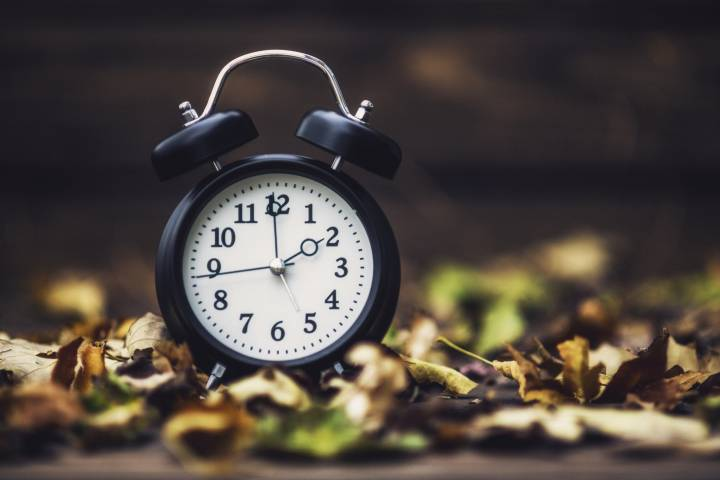
\includegraphics[width=0.2\linewidth]{2018/images/time.jpg}
  \caption{Time}
  \label{fig:time}
\end{figure}

Figure \ref{fig:time} shows a clock. Clocks always denote the passage of time. 
They have the ability to show what the current time is, and how quickly time
is moving compared to our own thoughts. Time is another interesting obstacle in 
this life. It has many different meanings to different people. But it is a 
showing of a passage as it were. A continuous moving section which doesn't stop 
or pause for anyone. It does not move in reverse either. It is constantly moving 
forward.